\label{key}\documentclass[letterpaper, 12pt,oneside]{article}
\usepackage{amsmath}
\usepackage{graphicx}
\usepackage{xcolor}
\graphicspath{{Imagenes/}}
\usepackage[utf8]{inputenc}
\usepackage{listings}
\usepackage[hidelinks]{hyperref}

\title{\Huge Taller de Herramientas Computacionales}
\author{Josué Artemio Hernández Rodríguez}
\date{24/Enero/2019}

\begin{document}
	\maketitle
	\begin{center}
		
\includegraphics[scale=0.7]{3.jpg}
	\end{center}

	\newpage
	
	\title{\huge \textit{Bitacora problema 2 }}\\
	
	El problema consistía que a partir de cierta altura, velocidad y una constante g, calcular los tiempos en que alcanza esa altura. Primero despeje la fórmula de segundo grado, para obtener t, y con la formula general tuve se tienen los dos valores t1 y t2 que se buscan. Solo definí la función como tiempo y coloque la fórmula en el bucle de la función, dos veces para obtener los valores t1 y t2, y que los regresara la función, es decir return t1, t2

	\begin{figure}[h]
		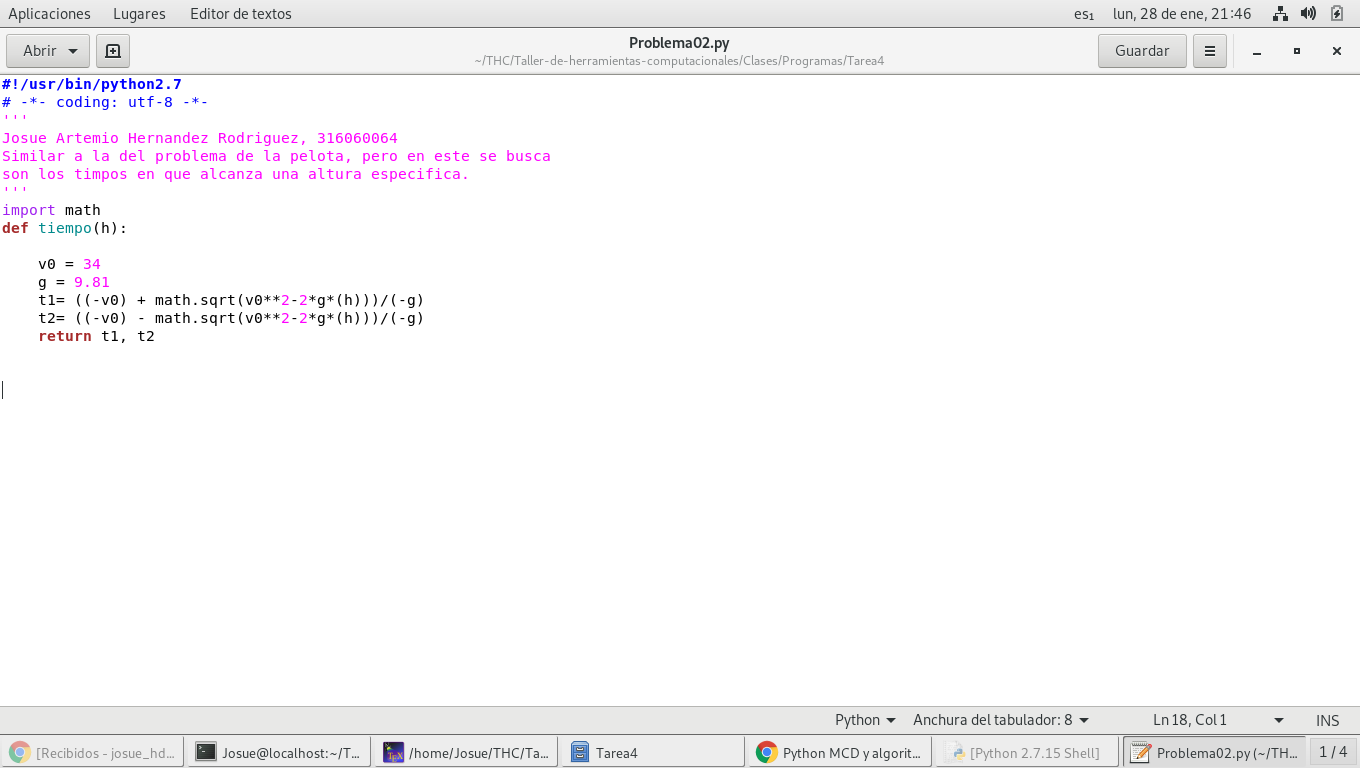
\includegraphics[scale=0.3]{pro02.png}
	\end{figure}
	
	
	
	
	
	
	
	
	
	
	
\end{document}
